\chapter{Plugins}
\index{Plugin}
\xirp~bietet ein \seegls{Framework} zur Pluginentwicklung mit welchem die Steuerung
eines Roboters realisiert werden kann.

Jedes \seegls{Plugin} ist dabei ein eigenes Jar mit einem bestimmen Aufbau, welches beim
Start von \xirp~erkannt und geladen wird. \seegls{Plugins} k�nnen im 
\index{Profil!Roboter}Roboter \seegls{Profil} einem
Roboter zugeordnet werden.

Die Plugin-\seegls{API} bietet dabei folgende Features:
\begin{itemize}
  \item Internationalisierung
  \item Bereitstellung von Funktionalit�t f�r die Toolbar
  \item Nutzung eigener Bilder
  \item \index{Einstellungen}Einstellungen f�r das \seegls{Plugin}
  \item Graphische Benutzeroberfl�che (eingebettet, in eigenem Fenster)
  \item Bereitstellung von Kommandos (und Steuerung �ber Tastatur/\seegls{Gamepad})
  \item Reporterstellung
  \item Nutzung von \seegls{Sensor}daten des Roboters
  \item Nutzung zus�tzlicher Java (Jars) und Nativer (\seegls{dll}/\seegls{so}) \seegls{Bibliothek}en
  \item Erstellung von \seegls{HTML}-Hilfe
  \item Implementierung der Kommunikation �ber eine Schnittelle (TCP/IP)
  \item Implementierung eines Kommunikationsprotokolls f�r einen Roboter 
\end{itemize}

In den Folgenden Abschnitten wird die Erstellung eines \seegls{Plugins} mit den
verschiedenen Features nach und nach beschrieben.

\section{Ein erstes Plugin}
\label{sec:firstplugin}
\index{Plugin!erstellen|(}
Voraussetzungen:
\begin{itemize}
\item Java (\seegls{JDK}) ab 1.6
\item Entwicklungsumgebung wie eclipse
\item \xirp~Installation
\end{itemize}

Der erste Schritt ist das erstellen eines neuen Projektes und hinzuf�gen des
\xirp~jar aus dem Installationsordner sowie
des \seegls{SWT} Jar aus dem Unterordner \fileQuote{lib/windows} oder \fileQuote{lib/linux} und hinzuf�gen.

Dann kann eine neue Klasse erstellt werden, welche
\index{Plugin!IPlugable!AbstractPlugin}
\newline\codeQuote{de.unibremen.rr.xirp.plugin.AbstractPlugin} erweitert (\refFig{newPluginClass}). \par
\kfig{plugin_plugin_newPluginClass}{1}{Erstellen einer neuen Pluginklasse}{newPluginClass}

Damit die Applikation wei�, dass diese neu erstellte Klasse die \index{Plugin!Hauptklasse}Hauptklasse 
des Plugins ist, muss eine \index{Plugin!Properties}properties Datei erstellt werden (\refFig{properties}).

Eine Vorlage dieser Properties Datei befindet sich bei der Installation im Ordner 
\fileQuote{development} als \fileQuote{plugin.properties.template}. Diese Datei in das Paket der 
\seegls{Plugin}-Klasse kopieren und die Endung \texttt{.template} entfernen.

\kfig{plugin_properties}{1}{Eine \enquote{plugin.properties}-Datei}{properties}

Nun k�nnen die Methoden mit Inhalten gef�llt werden.

Die Methode \index{Plugin!IPlugable!runInternal()}\codeQuote{runInternal()} 
wird ausgef�hrt wenn das Plugin gestartet wird. Um eine Ausgabe im 
Systemprotokoll von \xirp~zu erhalten muss noch eine Konstante f�r das 
\seegls{Logging} definiert werden.

Dies sieht wie folgt aus:
\codeQuote{private static final RobotLogger LOGGER = RobotLogger.getLogger(MyPlugin.class);}

Der \index{Roboter!Logging}\index{Logging!Roboter}\codeQuote{RobotLogger} ist im Paket 
\codeQuote{de.unibremen.rr.xirp.io.logging} zu finden. 

Die Ausgabe in 
\codeQuote{runInternal()} erfolgt dann �ber 
\codeQuote{LOGGER.info(robotName,''Ausgabe'');}. 

Die Methoden 
\index{Plugin!IPlugable!getPluginType()}\codeQuote{getPluginType()} gibt den 
Typ des Plugins zur�ck. Die \seegls{Plugin} Typen kommen aus der Klasse 
\index{Plugin!PluginType}\codeQuote{de.unibremen.rr.xirp.plugin.PluginType}. �hnliches
gilt f�r den 
\index{Plugin!VisualizationType}Darstellungstyp den die Methoden 
\index{Plugin!IPlugable!getVisualizationType()}\codeQuote{getVisualizationType()} 
zur�ckgibt.

Die Methoden 
\index{Plugin!IPlugable!getDescriptionKey()}\codeQuote{getDescriptionKey()} und 
\index{Plugin!IPlugable!getNameKey()}\codeQuote{getNameKey()} geben einen Schl�ssel 
zur \index{Internationalisierung!Schl�ssel}�bersetzung des \seegls{Plugin} Namens und der \seegls{Plugin} Beschreibung zur�ck.

\kfig{plugin_basicProperties}{1}{�bersetzungsdateien f�r ein Plugin}{basicProperties}

F�r die �bersetzung kommen nun noch zwei weitere Dateien 
(\refFig{basicProperties}) hinzu:\\
\index{Internationalisierung!Plugin}\fileQuote{messages$\_$de.properties} f�r 
die Deutsche �bersetzung und 
\index{Internationalisierung!Plugin}\fileQuote{messages$\_$en.properties} f�r 
die Englische �bersetzung.

Die entstandene Java-Klasse ist in \autoref{stubsFilled} zu sehen.

Das erste \seegls{Plugin} ist nun fast fertig. Nun muss nur noch ein Jar daraus erstellt
werden. Dazu kann aus dem Ordner \fileQuote{development} der Installation die \seegls{Ant}-\fileQuote{build.xml}
in den Hauptordner des Projekts kopiert werden.

Die Pfade oben in der \index{Ant!build.xml}\fileQuote{build.xml} m�ssen entsprechend angepasst werden. Dies 
betrifft normalerweise nur den Eintrag \codeQuote{plugins.pkg}.

Dann kann der Task \index{Ant!build.xml!singlePlugin}\codeQuote{singlePlugin} ausgef�hrt werden. Im Ordner \fileQuote{jar} liegt nun ein 
jar des \seegls{Plugins}. Dieses kann nun in die \xirp~Installation in den Ordner \fileQuote{plugins} 
kopiert werden.

Startet man nun \xirp~wird das \seegls{Plugin} geladen. Ob dies funktioniert hat kann man 
�ber das Men� \menuQuote{?} und den Eintrag \index{Men�!?!�ber Plugins}\menuQuote{�ber Plugins}
herausfinden. Wurde das \seegls{Plugin} 
geladen so ist es dort in der Tabelle aufgelistet (\refFig{aboutPlugins}).

\kfig{plugin_stubsFilled}{1}{Eine einfache Pluginklasse: MyPlugin.java}{stubsFilled}

\kfig{plugin_aboutPlugins}{1}{Men�: �ber Plugins}{aboutPlugins}

Damit das \seegls{Plugin} ausgef�hrt wird, muss es einem Roboter hinzugef�gt werden.

Dazu kann der Roboter \robotQuote{TesterBot} genutzt werden. Die Definition dieses Roboters 
befindet sich in der Installation \index{Profil!Roboter}\fileQuote{conf/profiles/robots/testerbot.bot}.

\newpage
Um das \seegls{Plugin} einzubinden muss einfach nur ein Element zum Element \codeQuote{plugins} ganz 
unten hinzugef�gt werden welches wie folgt aussieht:\index{Profil!Roboter!Plugin}

\begin{xml}[caption=Plugin in Roboterprofil eintragen,label=lst:smplplug:first:xml]
<plugin name="MeinPlugin">
	<class>xirp.plugins.MyPlugin</class>
	<usemultimedia>false</usemultimedia>
</plugin>
\end{xml}

Startet man \xirp~nun wieder kann man den Roboter \robotQuote{TesterBot} ausw�hlen und findet 
im Men� unter \index{Men�!Plugins}\menuQuote{Plugins} das eigene \seegls{Plugin} wieder. Klickt man darauf so wird das 
\index{Plugin!ausf�hren}\seegls{Plugin} ausgef�hrt und es sollte eine entsprechende Ausgabe im \index{Logging!Systemprotokoll}Systemprotokoll 
erscheinen.

\index{Plugin!erstellen|)}
\section{Die Toolbar}
\label{sec:plugin:toolbar}
\index{Toolbar}
Ein \seegls{Plugin} kann Funktionen auf die Toolbar des Roboters legen. Dazu 
muss der \seegls{Plugin} Typ auf 
\index{Plugin!PluginType}\codeQuote{PluginType.TOOLBAR} und der Darstellungstyp 
auf 
\index{Plugin!VisualizationType}\codeQuote{VisualizationType.ROBOT\_TOOLBAR} 
ge�ndert werden und die Methode 
\index{Plugin!IPlugable!getToolbar()}\codeQuote{getToolbar} �berschrieben 
werden.

Als Beispiel wird nun ein Button erstellt, welcher beim klicken einen Text
ausgibt.

Der Button soll ein \index{Bild!Icon}\seegls{Icon} statt Text haben. Daf�r wird ein neuer Ordner 
Namens \index{Plugin!Ordnerstruktur!images}\fileQuote{images} neben dem Ordner 
\index{Plugin!Ordnerstruktur!lib}\codeQuote{lib} im Plugin Paket angelegt in 
welchen ein \index{Bild!im Plugin}Bild \fileQuote{hallowelt.png} gelegt wird.
\index{Manager!ImageManager}
\begin{java}[caption=Eine Plugin Toolbar,
				 label=lst:smplplug:toolbar_plugin_getToolBar]
	@Override
	public XToolBar getToolBar(CoolItem parent) {
		XToolBar tools = new XToolBar(parent.getParent( ), SWT.FLAT);
		// �bersetzungshandler dieses Plugins mit �bergeben
		XToolItem helloWorld = new XToolItem(tools,
				SWT.FLAT | SWT.PUSH,
				handler);
		// Bild vom ImageManager holen
		helloWorld.setImage(ImageManager.getPluginImage(this, "helloworld.png")); //$NON-NLS-1$
		// Key f�r den Tooltip setzen
		helloWorld.setToolTipTextForLocaleKey("MyPlugin.toolbar.helloworld"); //$NON-NLS-1$
		helloWorld.addSelectionListener(new SelectionAdapter( ) {

			/*
			 * (non-Javadoc)
			 * 
			 * @see org.eclipse.swt.events.SelectionAdapter#widgetSelected(org.eclipse.swt.events.SelectionEvent)
			 */
			@Override
			public void widgetSelected(SelectionEvent e) {
				// �bersetzte Logausgabe mit einer Variablen
				LOGGER.info(robotName,
						getI18nString("MyPlugin.print.helloworld",
								MyPlugin.this.getRobotName( ))
								+ Constants.LINE_SEPARATOR);
			}
		});

		return tools;
	}
\end{java}

Wichtig ist das nicht die original \index{Widget}\seegls{SWT} Widgets benutzt 
werden sondern die aus dem Paket 
\newline\index{Widget!Custom}\codeQuote{de.unibremen.rr.xirp.ui.widgets.custom}. Sie 
bieten alle die Methoden 
\newline\index{Widget!Custom!setToolTipTextForLocaleKey()}\codeQuote{setToolTipTextForLocaleKey} 
und \index{Widget!Custom!setTextForLocaleKey()}\codeQuote{setTextForLocaleKey} 
(oder �hnliche) und einen Konstruktor der einen 
\index{Internationalisierung}�bersetzungshandler bekommen kann, mit welchem die 
\index{Internationalisierung!Schl�ssel}Schl�ssel letztendlich �bersetzt werden. 
Weiterhin �bernehmen all diese Custom Widgets immer die \index{Farbe}aktuellen 
Farb- und \index{Internationalisierung}Spracheinstellung auch bei einer 
�nderung im laufenden Betrieb.

Das hinzugef�gte Bild kann vom
\index{Manager!ImageManager}\codeQuote{de.unibremen.rr.xirp.
ui.util.ressource.ImageManager} abgerufen
werden. Dieser handelt auch das eigentlich n�tige \index{SWT!dispose}\seegls{disposen} des Bildes nach der
Benutzung und \seegls{cached} die Bilder, so dass von jedem nur eine Instanz existiert
die mehrfach genutzt werden kann.

\kfig{plugin_toolbar}{.7}{Toolbar Icon eines Plugins}{toolbar}

Auch der Text der beim klicken auf den Button ausgegeben wird, wird �bersetzt.
Dazu dient die Methode \codeQuote{getI18nString()} welche einen Schl�ssel und optional
noch mehrere Parameter zur Ersetzung von Variablen erhalten kann. Wichtig ist
 auch das abschlie�ende \codeQuote{Constants.LINE\_SEPARATOR} welches einen
Zeilenumbruch f�r das aktuelle Betriebssystem enth�lt.

So sehen die ver�nderten \index{Internationalisierung!Plugin}\fileQuote{properties}-Dateien aus:\\
\textbf{de}

\begin{properties}[caption=Deutsche �bersetzungen,
				 label=lst:smplplug:toolbar_props_de]
MyPlugin.plugin.name=Mein Plugin
MyPlugin.plugin.description=Ein Testplugin

MyPlugin.toolbar.helloworld=Hallo Welt ausgeben
MyPlugin.print.helloworld={0} sagt: "Hallo Welt!"
\end{properties}

\newpage
\textbf{en}
\begin{properties}[caption=Englische �bersetzungen,
				 label=lst:smplplug:toolbar_props_en]
MyPlugin.plugin.name=My Plugin
MyPlugin.plugin.description=A test plugin

MyPlugin.toolbar.helloworld=Print out Hello World
MyPlugin.print.helloworld={0} says: "Hello World!"
\end{properties}

Das \seegls{Plugin} kann nun wiederum mit der 
\index{Ant!build.xml}\fileQuote{build.xml} erstellt und in den Ordner 
\fileQuote{plugins} des \xirp~Installationsordners kopiert werden.



Bei der Ausf�hrung erscheint dann f�r den \robotQuote{TesterBot} ein \index{Bild!Icon}\seegls{Icon} auf der
Toolbar welches eine Weltkugel zeigt (\refFig{toolbar}). Dieses gibt bei einem Klick
\begin{lstlisting}
TesterBot: TesterBot sagt: "Hallo Welt!"
\end{lstlisting}

bzw.
\begin{lstlisting}
TesterBot: TesterBot says: "Hello World!"
\end{lstlisting}
\chapter{Einstellungen}
\index{Einstellungen|(}
\index{Plugins}
\label{ref:settings}

In \xirp~existiert eine einzelne Stelle, wenn es um Einstellungen f�r die
Anwendung und der darin geladenen Plugins geht, der Dialog 
\enquote{Einstellungen}. Die Einstellungen der Anwendung sind in die folgenden
neun Kategorien eingeteilt.

\begin{itemize}
  \item Allgemeine Einstellungen
  \item Erscheinungsbild
  \item Spracheinstellungen
  \item Tastenk�rzel
  \item Externe Werkzeuge
  \item Datenbankeinstellungen
  \item Maileinstellungen
  \item Speech-Einstellungen
  \item Diagrammeinstellungen
\end{itemize}

Jedes Plugin kann Einstellungen definieren. Wenn dies der Fall ist, erh�lt das
Plugin in einer Einstellungsgruppe des Roboters eine eigene Kategorie unter der
sich die Einstellungen des Plugins befinden. Das folgende Kapitel erl�utert alle
existierenden Einstellungsm�glichkeiten und gibt einen Einblick in den Dialog
mit dem diese Einstellungen get�tigt werden k�nnen.

\newpage

\section{Einstellungsdialog}

Der Dialog zum Vornehmen der systemweiten und pluginspezifischen Einstellungen
ist in einen Kategorie- und einen Inhaltsbereich aufgeteilt. Der
Kategoriebereich ist in Abbildung \ref{img:settings:dialog} auf Seite
\pageref{img:settings:dialog} rot und der Inhaltsbereich blau markiert.

\begin{figure}[ht]
    \centering
    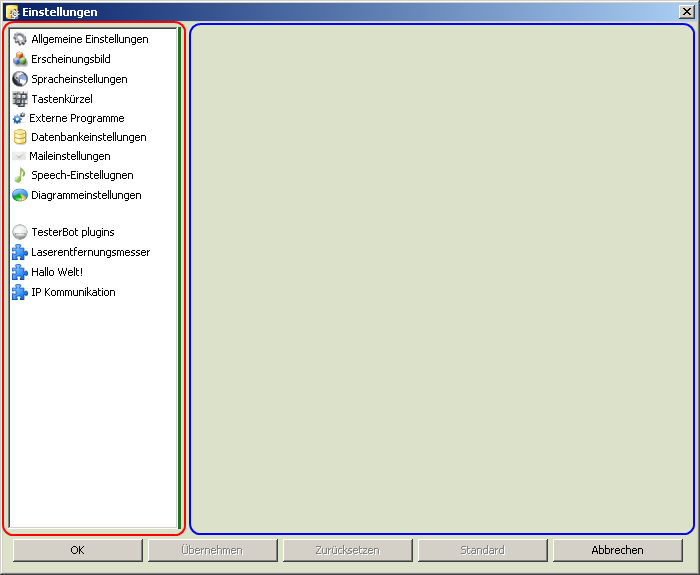
\includegraphics[width=1\textwidth]{images/settingsdialog}
    \caption{Der Settingsdialog mit markierten Kategorie- und Inhaltsbereichen}
    \label{img:settings:dialog}
\end{figure}

Um die Einstellungen einer Kategorie oder eines Plugins vorzunehmen, muss durch
einen Klick auf das entsprechende Listenelement auf der linken Seite der Inhalt
aufgerufen werden. In der Abbildung \ref{img:settings:content}
auf Seite \pageref{img:settings:content} ist der Inhalt f�r
\enquote{Allgemeinen Einstellungen} zu sehen.

\begin{figure}[hp]
    \centering
    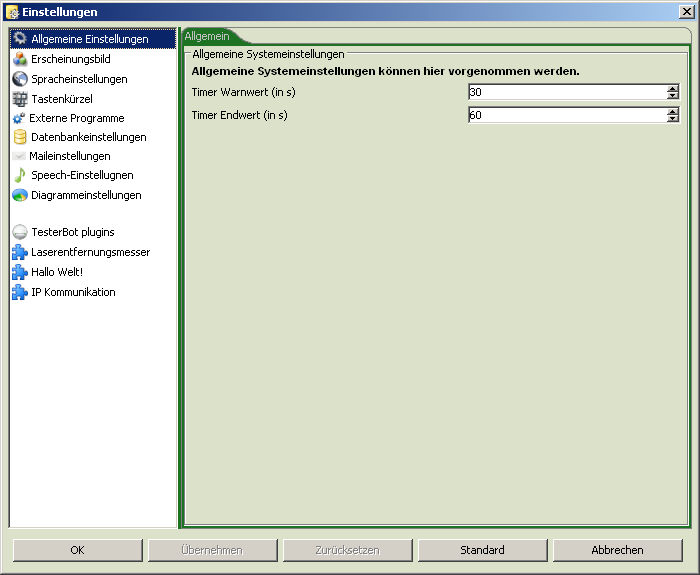
\includegraphics[width=1\textwidth]{images/settingscontent}
    \caption{Der Settingsdialog mit ge�ffnetem \enquote{Allgemeine Einstellungen}
    Inhalt}
    \label{img:settings:content}
\end{figure}

\newpage

Wie in den Abbildungen zu sehen gibt es diverse Kn�pfe die man anklicken k�nnte.

\begin{itemize}
  \item \texttt{OK}, speichert die neuen Einstellungen und schie�t den Dialog
  \item \texttt{�bernehmen}, speichert die neuen Einstellungen
  \item \texttt{Zur�cksetzen}, setzt auf den zuletzt gespeicherten Wert zur�ck
  \item \texttt{Standard}, setzt den Wert auf seinen Standard Wert
  \item \texttt{Abbrechen}, verwirft alle neuen Einstellungen und schlie�t den Dialog
\end{itemize}

\texttt{Zur�cksetzen} und \texttt{Standard} sind nur verf�gbar, wenn die Funktion
von den Einstellungen unterst�tzt wird.

In den folgenden Abschnitten werden die einzelnen Einstellungsm�glichkeiten der
Anwendung erl�utert.

\section{Allgemeine Einstellungen}
In den allgemeinen Einstellungen gibt es zwei Werte die einstellbar sind.

\begin{itemize}
  \item Timer Warnwert
  \item Timer Endwert
\end{itemize}

Die Werte f�r diese Einstellungen werden in Sekunden angegeben. Sie werden bei
der Farbberechnung der Stoppuhr Anzeige benutzt. Nach den im Warnwert
angegebenen Sekunden wechselt die Anzeige ihre Farbe nach orange. Wird der
Endwert erreicht, wechselt die Anzeige ihre Farbe nach rot.

\section{Erscheinungsbild}
In den Einstellungen f�r das Erscheinungsbild der Anwendung gibt es sieben
Farboptionen.

\begin{itemize}
  \item Reiterfarbe
  \item Reiterschriftfarbe
  \item Textfarbe eines inaktiven Reiters
  \item Farbe f�r diverse Elemente die den Fokus haben
  \item Trennlinienfarbe
  \item Hintergrundfarbe
  \item Farbe der Elementtitel
\end{itemize}

Eine Demonstration der Farbenwerte kann in Abbildung \ref{img:settings:badcolor}
auf Seite \pageref{img:settings:badcolor} betrachtet werden.

\begin{figure}[ht]
    \centering
    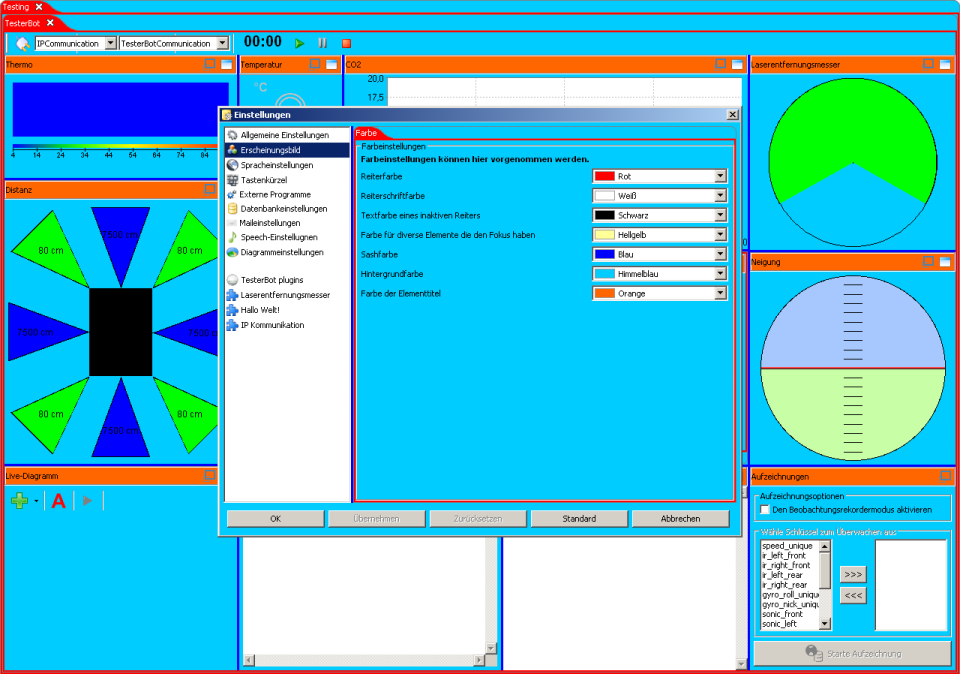
\includegraphics[width=1\textwidth]{images/badcolors}
    \caption{\xirp~mit abweichender Kolorierung zum Verdeutlichung der Farboptionen}
    \label{img:settings:badcolor}
\end{figure}

\section{Spracheinstellungen}
\index{Internationalisierung}
In den Spracheinstellungen gibt es nur eine Option: Die zu verwendende Sprache
der Anwendung. \xirp~unterst�tzt momentan die folgenden Sprachen. Weitere
Sprachpakete sollen in Zukunft folgen.

\begin{itemize}
  \item Deutsch
  \item Englisch
\end{itemize}

Die eingestellte Sprache gilt sowohl f�r die Anwendung als auch f�r die
geladenen Plugins. Sollte ein Plugin f�r die eingestellte Sprache keine
Sprachdatei zur Verf�gung stellen wird die Standard Sprache des Plugins
benutzt.

\section{Tastenk�rzel}
Die Kategorie \enquote{Tastenk�rzel} enth�lt zwei Typen von Tastenk�rzeln.

\begin{itemize}
  \item Anwendungsk�rzel, z.B. Strg+Q
  \item Kommandok�rzel
\end{itemize}

\subsection{Anwendungsk�rzel}
\index{Hotkey}
Die Anwendungsk�rzel werden benutzt um oft benutzte Funktionen mittels einer
Tastenkombination verf�gbar zu machen. In \xirp~gibt es diverse Tastenk�rzel. In
den Einstellungen gibt es eine Aufteilung nach den Tasten vor dem eigentlichen
\seegls{Hotkey}.

\begin{itemize}
  \item Strg+
  \item Strg+Umschalt+
  \item Strg+Alt+
\end{itemize}

F�r jede dieser 3 M�glichkeiten existiert ein eigener Reiter auf der Inhaltsseite
der Einstellungen. Die einzelnen verf�gbaren Funktionen werden im folgenden
erl�utert.

\newpage

\subsubsection{Strg+ - Tastenk�rzel}
\index{Hotkey}
Es existieren sieben Funktionen deren Tastenk�rzel frei bestimmt werden kann.
Der \enquote{\seegls{Hotkey}} wird nach der Steuerung-Taste (Strg) erwartet.

\begin{itemize}
  \item Programm beenden
  \item Einstellungen �ffnen
  \item Hilfe anzeigen
  \item Mailverwaltung �ffnen
  \item Konfigurationsdialog f�r den Diagrammgenerator �ffnen
  \item Reportsuche �ffnen
  \item Kontaktverwaltung �ffnen
\end{itemize}

\subsubsection{Strg+Umschalt+ - Tastenk�rzel}
\index{Hotkey}
Es existiert eine Funktion deren Tastenk�rzel frei bestimmt werden kann.
Der \enquote{\seegls{Hotkey}} wird nach der Steuerung- plus der Umschalt-Taste
(Strg+Umschalt) erwartet.

\begin{itemize}
  \item Programminformationen anzeigen
\end{itemize}

\subsubsection{Strg+Alt+ - Tastenk�rzel}
Es existiert eine Funktion deren Tastenk�rzel frei bestimmt werden kann.
Der \enquote{\seegls{Hotkey}} wird nach der Steuerung- plus der Alt-Taste
(Strg+Alt) erwartet.

\begin{itemize}
  \item Plugininformationen anzeigen
\end{itemize}

\subsection{Kommando Tastenk�rzel}
\index{Kommandos}
\index{Kommandos!kommandierbar}
\index{Gamepad}
Plugins k�nnen kommandierbar sein, das bedeutet, dass ein Plugin/eine Klasse
gewissen Funktionen f�r Kommandos freigeben kann. Zum Beispiel k�nnte eine
\enquote{Notaus} Funktion freigegeben werden. Um diese Funktion nutzen zu
k�nnen muss f�r die Funktion entweder eine Taste der Tastatur, eine Taste eines
\seegls{Gamepad}s, oder beides hinterlegt werden. Dies kann in dem Inhaltsreiter
\enquote{Kommando Tastenk�rzel} getan werden. Die dort vorhandene Tabelle
enth�lt alle verf�gbaren Kommando-Funktionen (Siehe Abbildung
\ref{img:settings:commads} auf Seite \pageref{img:settings:commads}).

\begin{figure}[hbp]
    \centering
    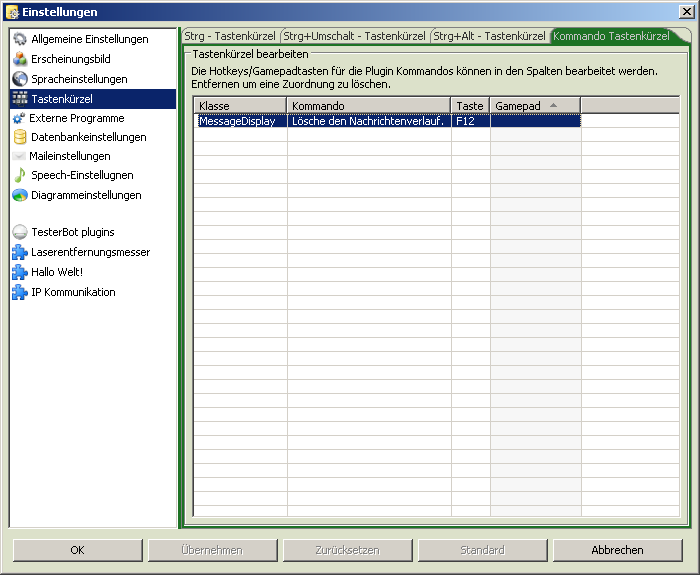
\includegraphics[width=1\textwidth]{images/commands}
    \caption{Kommando Tastenk�rzel Konfiguration}
    \label{img:settings:commads}
\end{figure}

Wie zu sehen ist, wurde der Funktion \enquote{L�sche den Nachrichtenverlauf.}
der Klasse \enquote{MessageDisplay} die Tastaturtaste \enquote{F12} zugewiesen.
Eine Gamepadtaste wurde noch nicht zugewiesen. Um nun die Taste zu �ndern oder
hinzuzuf�gen muss nur auf die entsprechende Tabellenzelle geklickt werden. Hier
�ffnet sich nun ein Eingabefeld. Dann muss nur noch die gew�nschte
Tastatur-/Gamepadtaste gedr�ckt werden.

\section{Externe Werkzeuge}
\index{Externe Werkzeuge}
In den Einstellungen f�r die externen Programme der \seegls{Profile} gibt es pro
geladenem Profil einen Inhaltsreiter. Jeder dieser Reiter enth�lt die
Konfigurationsoberfl�che die in Abbildung \ref{img:settings:ext} auf Seite
\pageref{img:settings:ext} zu sehen ist.

\begin{figure}[hp]
    \centering
    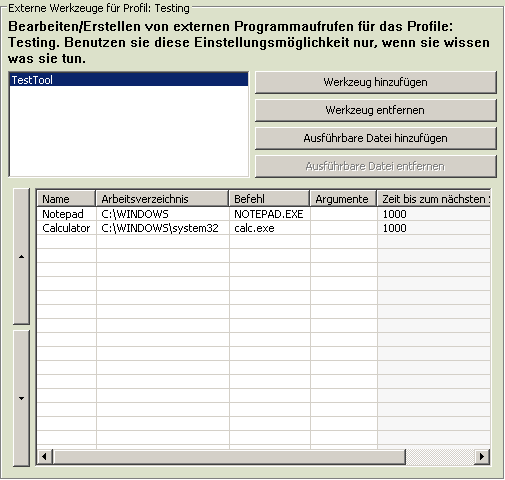
\includegraphics[width=.75\textwidth]{images/ext}
    \caption{Oberfl�che zum konfigurieren der externen Programme}
    \label{img:settings:ext}
\end{figure}

Um ein neues externes Werkzeug anzulegen muss einfach auf den Knopf
\enquote{Werkzeug hinzuf�gen} geklickt werden. Dann muss in dem folgenden
Eingabedialog der Name des Werkzeugs angegeben werden. Ist dies erfolgreich
wird in der List das neue Werkzeug angezeigt. Der n�chste Schritt ist nun diesem
Werkzeug mindestens ein ausf�hrbares Programm zuzuordnen. Dazu muss zuerst das
Werkzeug in der Liste markiert werden und dann auf den Knopf
\enquote{Ausf�hrbare Datei hinzuf�gen} geklickt werden.
\par
Der folgende Eingabedialog erwartet zwei Pflichtangaben: Den Namen des Programms
und die Wartezeit nach Start der Anwendung. Der Name des Programms ist frei
w�hlbar. In dem Beispiel in Abbildung \ref{img:settings:ext:example} auf Seite
\pageref{img:settings:ext:example} ist als Name \enquote{Firefox} gew�hlt. Die
Wartezeit nach dem Start wird in Millisekunden angegeben. Dieser Wert kann
genutzt werden, um einem Programm eine gewissen zeitlichen Spielraum zu
verschaffen, bis ein weiteres gestartet wird. Dies ist n�tzlich falls
nachfolgende Programme von vorherigen abh�ngig sind.

\begin{figure}[hp]
    \centering
    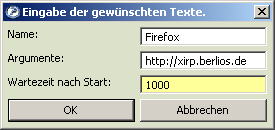
\includegraphics[width=0.5\textwidth]{images/ext_example}
    \caption{Beispieleingabe f�r ein ausf�hrbares Programm}
    \label{img:settings:ext:example}
\end{figure}

Die \enquote{Argumente} Eingabe ist optional. Hier k�nnen Argumente angegeben
werden die ein Programm beim Start ben�tigt. Wird dieser Eingabedialog best�tigt
erscheint ein Dateiauswahldialog. Erst jetzt wird die eigentliche ausf�hrbare
Datei ausgew�hlt.
\par
Wurden zu einem Werkzeug mehrere Programme hinzugef�gt kann die Reihenfolge in
der sie gestartet werden sollen mittels der Pfeiltasten auf der linken Seiten
ver�ndert werden.

\section{Datenbankeinstellungen}
\index{Datenbank}
In den Einstellungen f�r die Datenbank gibt es f�nf Optionen die eingestellt
werden k�nnen.

\begin{itemize}
  \item IP-Adresse
  \item Port
  \item Benutzer
  \item Passwort
  \item Datenbanktreiber
\end{itemize}

\newpage

Die ersten vier Optionen beziehen sich auf Datenbanken die �ber \seegls{TCP/IP}
kommunizieren. Diese sollten angegeben werden, wenn ein Datenbanktreiber gew�hlt
wird der diese Einstellungen ben�tigt. Momentan werden die folgenden Datenbanken
unterst�tzt.

\begin{itemize}
  \item HSQLDB
  \item MySQL
\end{itemize}

\index{Rekorder}
\index{Reporte}
Die \enquote{HSQSLDB} wird bei der Installation von \xirp~mitgeliefert, so dass
kein spezieller Datenbankserver vorhanden sein muss, um Aufzeichnungen mit dem
Rekorder vorzunehmen und Reporte abzuspeichern.

\section{Maileinstellungen}
\index{Mail}
In den Einstellungen f�r das Mailsystem gibt es sechs Optionen die eingestellt
werden k�nnen.

\begin{itemize}
  \item SMTP-Host
  \item Port
  \item Authentifizierung n�tig
  \item Benutzername
  \item Passwort
  \item No-Reply Adresse
\end{itemize}

Hier k�nnen die f�r die Kommunikation mit dem SMTP-\seegls{Server} n�tigen Einstellungen
gemacht werden. Die \enquote{No-Reply} Adresse muss gesetzt werden, da sonst das
Versenden von E-Mails nicht funktionieren wird.

\section{Speech-Einstellungen}
\index{Text-To-Speech}
\index{Sprachausgabe}
In den Einstellungen f�r das Speech-System\footnote{Bisher wird nur
Sprachausgabe unterst�tzt. Spracherkennung soll in einer zuk�nftigen Version
hinzukommen} gibt es zwei Optionen die eingestellt werden k�nnen.

\begin{itemize}
  \item Stimme der Sprachausgabe
  \item Sprachausgabe aktivieren
\end{itemize}

Die erste Option bestimmt die Stimme die f�r die Sprachausgabe benutzt werden
soll. Es gibt zwei Standard Sprachen:

\begin{itemize}
  \item kevin
  \item kevin16
\end{itemize}

Das Sprachausgabesystem unterst�tzt \enquote{MBROLA} Stimmen. Wenn diese
installiert werden, werden die neu hinzugekommenen Stimmen ebenfalls hier zur
Auswahl gestellt. in Kapitel \ref{ref:speech} ab Seite \pageref{ref:speech} kann
nachgelesen werden, wie diese zus�tzlichen Stimmen installiert werden k�nnen und
woher man diese beziehen kann.

\section{Diagrammeinstellungen}
\label{ref:settings:livechart}
\index{Live-Diagramme}
\index{Live-Diagramme!PDF}
\index{Live-Diagramme!PNG}
\index{Live-Diagramme!JPG}
\index{Live-Diagramme!CSV}
In den Einstellungen f�r die Live-Diagramme gibt es vier Optionen die eingestellt
werden k�nnen. Alle beziehen sich darauf, ob nach dem Stoppen eines
Plottingvorgangs das erzeugte Diagramm in verschiedenen Formaten automatisch
exportiert werden sollen.

\begin{itemize}
  \item PDF beim Stoppen eines Live-Diagramms automatisch exportieren
  \item PNG beim Stoppen eines Live-Diagramms automatisch exportieren
  \item JPG beim Stoppen eines Live-Diagramms automatisch exportieren
  \item CSV beim Stoppen eines Live-Diagramms automatisch exportieren
\end{itemize}

\index{Einstellungen|)}

\section{Benutzeroberfl�che}
\index{Plugin!Benutzeroberfl�che!erstellen|(}
Bisher hat das kleine Beispielplugin noch keine eigene Oberfl�che, wenn man von
dem \index{Bild!Icon}\seegls{Icon} in der \index{Toolbar}Toolbar einmal absieht. Dies soll sich nun �ndern.

F�r die Oberfl�che wird eine neue Klasse ben�tigt die
\index{Plugin!Benutzeroberfl�che!AbstractPluginGUI}\codeQuote{AbstractPluginGUI} erweitert.

Die \index{Plugin!Hauptklasse}Basisklasse des \seegls{Plugins} \codeQuote{MyPlugin} ist eine Klasse die
\index{generisch}\seegls{generisch} ist und eigentlich \index{generisch!Typparameter}\seegls{Typparameter} ben�tigt. Diese wurden bisher zur
Vereinfachung weggelassen, werden nun aber ben�tigt. Die Klasse
\codeQuote{MyPlugin} ist wie in \autoref{basicGUI} zu sehen zu erweitern.

\kfig{plugin_basicGUI}{1}{Generische Typen in der Pluginklasse einstellen}{basicGUI}

Nun muss in \codeQuote{MyPlugin} die Methode \index{Plugin!IPlugable!getGUIInternal()}\codeQuote{getGUIInternal()}
�berschrieben werden, so dass sie eine neue Instanz von \codeQuote{MyPluginGUI} zur�ckgibt.

\begin{java}[caption=Oberfl�che aus Plugin zur�ckgeben,
				 label=lst:smplplug:gui_gui_getGUIInternal]
	@Override
	protected MyPluginGUI getGUIInternal(Composite parentPanel) {
		return new MyPluginGUI(parentPanel, this);
	}
\end{java}

Nun muss noch \xirp~mitgeteilt werden, dass dieses \seegls{Plugin} nun eine eigene
Oberfl�che besitzt. Dazu wird die R�ckgabe von
\index{Plugin!IPlugable!getVisualizationType()}\codeQuote{getVisualizationType()} ver�ndert:

\begin{java}[caption=Visualisierungstyp eines Plugin setzen,
				 label=lst:smplplug:gui_gui_getVisualizationType]
	@Override
	public int getVisualizationType() {
		return VisualizationType.ROBOT_TOOLBAR | VisualizationType.WINDOW;
	}
\end{java}
\index{Manager!ColorManager}
\index{Manager!FontManager}
Nun muss nur noch die Oberfl�che selbst ein wenig mit Leben gef�llt werden:
\begin{java}[caption=Beispiel Plugin-Oberfl�che,
				 label=lst:smplplug:gui_gui_sample]
package xirp.plugins;

import org.eclipse.swt.SWT;
import org.eclipse.swt.layout.GridData;
import org.eclipse.swt.widgets.Composite;

import de.unibremen.rr.xirp.plugin.AbstractPluginGUI;
import de.unibremen.rr.xirp.ui.util.SWTUtil;
import de.unibremen.rr.xirp.ui.util.ressource.ColorManager;
import de.unibremen.rr.xirp.ui.util.ressource.FontManager;
import de.unibremen.rr.xirp.ui.widgets.custom.XLabel;

public class MyPluginGUI extends AbstractPluginGUI {

	private MyPlugin plugin;

	public MyPluginGUI(Composite parent, MyPlugin plugin) {
		super(parent, plugin);
		this.plugin = plugin;
		init( );
	}

	private void init() {
		SWTUtil.setGridLayout(this, 3, true);
		setBackground(ColorManager.getColor(255, 0, 0));
		XLabel first = new XLabel(this, SWT.NONE, plugin.getHandler( ));
		first.setTextForLocaleKey("MyPluginGUI.firstLabel");
		SWTUtil.setGridData(first,
				true,
				true,
				GridData.CENTER,
				GridData.CENTER,
				1,
				1);

		XLabel second = new XLabel(this, SWT.NONE, plugin.getHandler( ));
		second.setTextForLocaleKey("MyPluginGUI.secondLabel");
		second.setFont(FontManager.getFont("Arial", 12, SWT.BOLD));
		SWTUtil.setGridData(second,
				true,
				true,
				GridData.FILL,
				GridData.CENTER,
				2,
				2);
	}
}
\end{java}

Hier werden 4 weitere neue Methoden gezeigt:
\begin{itemize}
\item Das erstellen von Farben mit dem \index{Manager!ColorManager}\codeQuote{ColorManager}. Diese m�ssen
nicht \index{SWT!dispose}\seegls{disposed} werden.
\item Das erstellen von Schriften mit dem \index{Manager!FontManager}\codeQuote{FontManager}. Diese m�ssen
ebenfalls nicht \seegls{disposed} werden.
\item Zuweisen eines Layout mit \index{SWTUtil!setGridLayout()}\codeQuote{SWTUtil.setGridLayout()}
\item Das zuweisen von Layout Daten mit \index{SWTUtil!setGridData()}\codeQuote{SWTUtil.setGridData()}
\end{itemize}

Das \seegls{Plugin} ist nun im \index{Men�!Plugins}\menuQuote{Plugins}-Men� zu finden und zeigt einen roten
Hintergrund mit zwei Texten (\refFig{GUITest}).

\kfig{plugin_GUITest}{1}{Eine kleine Benutzeroberfl�che f�r ein Plugin}{GUITest}

Damit das \seegls{Plugin} innerhalb des \index{Workspace}\seegls{Workspaces} des Roboters angezeigt wird
und nicht �ber das Men� aufgerufen werden muss, muss nur der Visualisierungtyp
von \codeQuote{WINDOW} auf \codeQuote{EMBEDDED} ge�ndert werden.
\index{Plugin!Benutzeroberfl�che!erstellen|)}
\section{Daten und Oberfl�che}
\index{Plugin!Plugindaten!erstellen|(}
Ein \seegls{Plugin} kann mehrere Oberfl�chen haben, die jedoch immer das selbe anzeigen
sollen. Dies resultiert daraus, dass eine Oberfl�che z.B. in der �bersicht des
Roboters und eine Zweite in der Gesamt�bersicht aller Roboter zu sehen ist.

Damit diese nun das gleiche Anzeigen besteht die M�glichkeit diese �ber eine
Datenklasse zu synchronisieren.

Auch f�r das \seegls{Plugin} selbst bietet sich so eine bessere Steuerung der Oberfl�che.
Es braucht nur die Daten zu setzen und die Oberfl�che zeigt diese dann
an. 

Um Daten zu nutzen, muss eine neue Klasse \codeQuote{MyPluginData} erstellt 
werden, welche \index{Plugin!Plugindaten!AbstractData}\codeQuote{AbstractData} 
erweitert.

Dem Konstruktor sollte direkt einen Parameter f�r die Plugin Basisklasse
hinzugef�gt werden:
\begin{java}[caption=Plugindaten erstellen,label=lst:smplplug:data:newclass]
package xirp.plugins;

import de.unibremen.rr.xirp.plugin.AbstractData;

public class MyPluginData extends AbstractData {

	private MyPlugin plugin;

	public MyPluginData(MyPlugin plugin) {
		super( );
		this.plugin = plugin;
	}
}
\end{java}

In der Klasse \codeQuote{MyPlugin} kann nun der \index{generisch!Typparameter}\seegls{generische} \seegls{Typparamter} \codeQuote{AbstractData}
durch \codeQuote{MyPluginData} ersetzt werden:
\begin{java}[caption=Plugindaten in Plugin eintragen,label=lst:smplplug:data:plugin_extends]
public class MyPlugin extends AbstractPlugin<MyPluginData, MyPluginGUI> {
...
}
\end{java}

Nun kann die Methode \index{Plugin!IPlugable!getPluginDataInternal()}\codeQuote{getPluginDataInternal()} �berschrieben werden:
\begin{java}[caption=Plugindaten aus Plugin zur�ckgeben,label=lst:smplplug:data:plugin:getPluginDataInternal]
	@Override
	protected MyPluginData getPluginDataInternal() {
		return new MyPluginData(this);
	}
\end{java}

Nun wird der \codeQuote{MyPluginData} ein Feld \codeQuote{toPrint} und
entsprechende Getter und Setter hinzugef�gt. Der eigentliche Setter muss nun ein wenig
modifiziert werden, so dass er beim Aufruf eine \index{Plugin!Plugindaten!notifyUI()}Benachrichtigung sendet, dass
sich Daten ge�ndert haben.

\begin{java}[caption=Methoden in Plugindaten hinzuf�gen
,label=lst:smplplug:data:data:methods]
public class MyPluginData extends AbstractData {

	private MyPlugin plugin;
	private String toPrint;

	public MyPluginData(MyPlugin plugin) {
		super( );
		this.plugin = plugin;
	}

	public String getToPrint() {
		return toPrint;
	}

	public void setToPrint(String toPrint) {
		plugin.notifyUI("toPrint", this.toPrint, this.toPrint = toPrint);
	}
}
\end{java}

Die Oberfl�che soll nun ein Textfeld anzeigen:
\begin{java}[caption=Oberfl�che zur Plugindatendarstellung,label=lst:smplplug:data:gui:init]
	private void init() {
		GridLayout gl = SWTUtil.setGridLayout(this, 1, true);
		SWTUtil.resetMargins(gl);

		this.setBackground(ColorManager.getColor(SWT.COLOR_RED));

		text = new XText(this, SWT.READ_ONLY | SWT.WRAP, false);
		SWTUtil.setGridData(text,
				true,
				true,
				GridData.FILL,
				GridData.FILL,
				1,
				1);

	}
\end{java}

Der Hintergrund der Oberfl�che ist eigentlich Rot, jedoch nimmt das Textfeld
durch die \codeQuote{FILL}-Attribute und das entfernen von R�ndern mit
\index{SWTUtil!resetMargins()}\codeQuote{SWTUtil.resetMargins()} den gesamten verf�gbaren Platz ein.
\par
Damit dieses Textfeld �nderungen der Daten verarbeitet fehlt noch eine neue
Methode welche im Konstruktor aufgerufen wird: 
\begin{java}[caption=Listener der Oberfl�che auf Plugindaten,label=lst:smplplug:data:gui:listener]
	public MyPluginGUI(Composite parent, MyPlugin plugin) {
		super(parent, plugin);
		this.plugin = plugin;
		init( );
		initListener( );
	}

	private void initListener() {
		MyPluginData pluginData = this.plugin.getPluginData( );
		pluginData.addPropertyChangeListener("toPrint",
				new PropertyChangeListener( ) {

					@Override
					public void propertyChange(PropertyChangeEvent event) {
						text.append(event.getNewValue( ).toString( ));
					}

				});
	}
\end{java}

In dieser Methode erfolgt die Anmeldung auf �nderungen der Eigenschaft
\codeQuote{toPrint} der \seegls{Plugin} Daten. �ndern sich die Daten, so wird dies im
Textfeld ausgegeben.

Nun fehlt noch das schreiben der Daten beim klicken auf das \index{Toolbar}Toolbar 
\index{Bild!Icon}\seegls{Icon}. Hierzu muss die Methode 
\index{Plugin!IPlugable!getToolbar()}\codeQuote{getToolbar()} ge�ndert werden.

\begin{java}[caption=Setzen von Plugindaten aus der Oberfl�che,label=lst:smplplug:data:gui:toolbar]
	@Override
	public XToolBar getToolBar(CoolItem parent) {
		XToolBar tools = new XToolBar(parent.getParent( ), SWT.FLAT);
		XToolItem helloWorld = new XToolItem(tools,
				SWT.FLAT | SWT.PUSH,
				handler);
		helloWorld.setToolTipTextForLocaleKey("MyPlugin.toolbar.helloworld"); //$NON-NLS-1$
		helloWorld.setImage(ImageManager.getPluginImage(this, "helloworld.png")); //$NON-NLS-1$
		helloWorld.addSelectionListener(new SelectionAdapter( ) {

			/*
			 * (non-Javadoc)
			 * 
			 * @see org.eclipse.swt.events.SelectionAdapter#widgetSelected(org.eclipse.swt.events.SelectionEvent)
			 */
			@Override
			public void widgetSelected(SelectionEvent e) {
				String string = getI18nString("MyPlugin.print.helloworld",
						MyPlugin.this.getRobotName( ),
						toPrint)
						+ Constants.LINE_SEPARATOR;
				LOGGER.info(robotName, string);
				pluginData.setToPrint(string);
			}
		});

		return tools;
	}
\end{java}

Immer wenn die Sprache umgestellt wurde oder in den \index{Einstellungen}Einstellungen ein neuer Text
f�r das \seegls{Plugin} gesetzt wurde, erscheint die Ausgabe beim Klick auf das Toolbar
\seegls{Icon} nun auch in der Oberfl�che des \seegls{Plugins} (\refFig{dataOut}). 

\kfig{plugin_dataOut}{.7}{Ausgabe in der Plugin Oberfl�che}{dataOut}
\index{Plugin!Plugindaten!erstellen|)}
\section{Synchronisation mit Daten}
\index{Plugin!Plugindaten!synchronisieren mit Oberfl�che}
\index{Plugin!Benutzeroberfl�che!synchronisieren mit Plugindaten}
Noch einfacher als das zuvor gezeigte Beispiel ist die Synchronisation von
\index{Widget}Widgets mit den Daten eines \seegls{Plugins}.
\par
Um dies zu Testen wird nun ein weiteres Feld zu den \index{Plugin!Plugindaten!notifyUI()}Daten hinzugef�gt:
\begin{java}[caption=Plugindaten notifizieren GUI,label=lst:smplplug:datasync:data:notifyUI]
	private int clickCount;

	public int getClickCount() {
		return clickCount;
	}

	public void setClickCount(int clickCount) {
		plugin.notifyUI("clickCount",
				this.clickCount,
				this.clickCount = clickCount);
	}

	public void incrementClickCount() {
		plugin.notifyUI("clickCount",
				this.clickCount,
				this.clickCount = clickCount + 1);
	}
\end{java}

Im \seegls{Plugin} wird nun zus�tzlich bei jedem Klick auf das \index{Bild!Icon}\seegls{Icon} noch
\codeQuote{incrementClickCount()} aufgerufen.

\begin{java}[caption=Plugindaten aus GUI setzen,label=lst:smplplug:datasync:gui:listener]
	helloWorld.addSelectionListener(new SelectionAdapter( ) {

			/*
			 * (non-Javadoc)
			 * 
			 * @see org.eclipse.swt.events.SelectionAdapter#widgetSelected(org.eclipse.swt.events.SelectionEvent)
			 */
			@Override
			public void widgetSelected(SelectionEvent e) {
				// �bersetzte Logausgabe mit einer Variablen
				String string = getI18nString("MyPlugin.print.helloworld",
						MyPlugin.this.getRobotName( ),
						toPrint)
						+ Constants.LINE_SEPARATOR;
				LOGGER.info(robotName, string);
				pluginData.setToPrint(string);
				pluginData.incrementClickCount( );

			}
		});
\end{java}

Um die Anzahl der Klicks in der \seegls{GUI} darzustellen kommen nun zum Textfeld
noch ein \codeQuote{Slider} und ein \codeQuote{Spinner} hinzu:
\index{Manager!ColorManager}
\begin{java}[caption=Oberfl�che mit Plugindaten synchronisieren,label=lst:smplplug:datasync:gui:sync]
	private void init() {
		GridLayout gl = SWTUtil.setGridLayout(this, 2, true);
		SWTUtil.resetMargins(gl);
		SWTUtil.resetSpacings(gl);

		this.setBackground(ColorManager.getColor(SWT.COLOR_RED));

		text = new XText(this, SWT.READ_ONLY | SWT.WRAP, false);
		SWTUtil.setGridData(text,
				true,
				true,
				GridData.FILL,
				GridData.FILL,
				2,
				1);

		XStyledSpinner spinner = new XStyledSpinner(this, SWT.NONE);
		sync(spinner, "clickCount");
		SWTUtil.setGridData(spinner,
				false,
				false,
				GridData.CENTER,
				GridData.CENTER,
				1,
				1);

		Slider slider = new Slider(this, SWT.NONE);
		sync(slider, "clickCount");
		SWTUtil.setGridData(slider,
				true,
				false,
				GridData.FILL,
				GridData.CENTER,
				1,
				1);
	}
\end{java}

Diese beiden \index{Widget}Widgets k�nnen einfach durch den Aufruf von \index{Plugin!Benutzeroberfl�che!sync()}\codeQuote{sync()} mit
dem entsprechenden Propertynamen mit den Daten synchronisiert werden.
\par
Beim Klicken auf das \index{Bild!Icon}\seegls{Icon} �ndern sich nun die Werte von \codeQuote{Slider} und
\codeQuote{Spinner}. Bewegt man den \codeQuote{Slider} �ndert sich auch der Wert
des \codeQuote{Spinner} und umgekehrt (\refFig{dataSync}).

\kfig{plugin_dataSync}{.7}{Synchronisation von Slider und Spinner}{dataSync}

\section{Kommandos}
\label{sec:plugin:commands}
\index{Kommando}
\index{Kommando!Manager}
Um ein \seegls{Plugin} per Tastatur oder \index{Gamepad}\seegls{Gamepad} steuerbar zu machen kann zus�tzlich noch
das Interface \codeQuote{de.unibremen.rr.xirp.io.command.ICommandable.java}
implementieren.

Im Beispielplugin soll so per Tastaturdruck der Klickz�hler erh�ht werden.

Nach folgendem Schema k�nnen Kommandos sehr einfach f�r \seegls{Plugins} implementiert werden:
\index{Manager!CommandManager}
\begin{java}[caption=Kommandodefinition im Beispielplugin,label=lst:smplplug:commands]
	@Override
	protected void runInternal() {
		readSettings( );
		CommandManager.register(this, robotName);
	}

	private static final String INCREMENT_CLICK_KEY = "MyPlugin.command.incrementClick";

	@Override
	public boolean executeCommand(Command command) {
		String key = command.getCommandDefinition( ).getKey( );
		boolean executed = false;
		if (key.equalsIgnoreCase(INCREMENT_CLICK_KEY)) {
			pluginData.incrementClickCount( );
			executed = true;
		}
		return executed;
	}


	private CommandDefinition getCommandDefinition(String key) {
		List<String> parameterNames = Collections.emptyList( );
		List<GeneratorType> types = Arrays.asList(GeneratorType.values( ));
		CommandDefinition def = new CommandDefinition(this,
				key,
				parameterNames,
				types,
				this.handler);
		return def;
	}

	@Override
	public List<CommandDefinition> getCommandDefinitions() {
		List<CommandDefinition> commandDefs = new ArrayList<CommandDefinition>( );
		commandDefs.add(getCommandDefinition(INCREMENT_CLICK_KEY));

		return commandDefs;
	}
\end{java}

Der Schl�ssel muss zu den \index{Internationalisierung!Schl�ssel}�bersetzungen hinzugef�gt werden. Er beschreibt in Kurzform
was das Kommando tut. Wichtig ist, das \seegls{Plugin} in \codeQuote{runInternal()} beim
\codeQuote{CommandManager} zu registrieren.

\index{Hotkey}
In \xirp~l�sst sich nun in den \index{Einstellungen!Hotkey}Einstellungen im Bereich \menuQuote{Tastenk�rzel}
auf dem Tab \menuQuote{Kommando Tastenk�rzel} auf der Tastatur eine Taste
eintippen die f�r das Kommando benutzt werden soll (\refFig{commandView}). 
Speichert und schlie�t man diese Einstellungen, so l�sst sich das \seegls{Plugin} nun mit
der eingestellten Taste tats�chlich steuern.

\kfig{plugin_commandView}{1}{Hotkeys f�r Kommandos einstellen}{commandView}
\section{Reporte Erstellen}
\label{sec:plugin:report}
\index{Report}

Die \seegls{Plugin}-\seegls{API} bietet auch die M�glichkeit so genannte Reports zu erstellen. Dies
sind \seegls{PDFs} welche selbst zusammengestellt werden k�nnen.

F�r das Beispielplugin kann so zum Beispiel die Anzahl der erfolgten Klicks
zusammen mit einem Screenshot der aktuellen Oberfl�che ausgegeben werden.

Dazu muss das \seegls{Plugin} als Typ zus�tzlich \codeQuote{PluginType.REPORT}
zur�ckgeben. Weiterhin m�ssen die Methoden \codeQuote{getReport()} und
\codeQuote{hasReport()} implementiert werden:
\index{Manager!ProfileManager}
\begin{java}[caption=Reporterstellung eines Plugins,label=code:plugin:report]
@Override
public int getPluginType() {
	return PluginType.TOOLBAR | PluginType.REPORT;
}

@Override
public boolean hasReport() {
	return pluginData.getClickCount( ) > 0;
}

@Override
public Report getReport() {
	Report r = null;
	try {
		Header h = new Header("Klickz�hler",
				ProfileManager.getRobot(robotName),
				this);
		Content c = new Content( );
		ContentPart part = new ContentPart( );
		ContentPartText text = new ContentPartText( );
		ContentPartTextParagraph para = new ContentPartTextParagraph( );
		para.setHeader("Klickanzahl");
		para.setText("In diesem Plugin wurde " +
				pluginData.getClickCount( ) + " mal geklickt.");
		text.addParagraph(para);
		part.addReportText(text);

		if (!guis.isEmpty( )) {
			MyPluginGUI gui = guis.firstElement( );
			Image image = gui.captureScreenshot( );
			ImageLoader loader = new ImageLoader( );
			loader.data = new ImageData[] {image.getImageData( )};
			String imagePath = Constants.TMP_DIR + Constants.FS +
					getClass( ).getName( ) + ".png";
			loader.save(imagePath, SWT.IMAGE_PNG);
			image.dispose( );

			ContentPartImage imagePart = new ContentPartImage(imagePath,
					"Screenshot der aktuellen GUI");

			part.addReportImage(imagePart);
		}

		c.addReportPart(part);
		r = new Report(h, c, h.getTitle( ));
	}
	catch (Exception e) {
		LOGGER.error(robotName, "Error: " + e.getMessage( ) +
				Constants.LINE_SEPARATOR, e);
	}
	return r;
}
\end{java}

Der Report soll nur erstellt werden, wenn �berhaupt schon einmal geklickt wurde.

F�r die Erstellung des Screenshot kann die Methode \codeQuote{captureScreenshot}
der Oberfl�che genutzt werden. Es reicht dabei einen Screenshot von einer
Oberfl�che zu nehmen (in diesem Fall der ersten), da diese ja alle das selbe
anzeigen.

\kfig{plugin_report_menu}{.5}{Plugin im Reportmen�}{img:plugin:report}

Das Bild muss vor der Einbindung in das \seegls{PDF} mit dem \codeQuote{ImageLoader} 
gespeichert werden, damit es
von einem Pfad direkt bei der \seegls{PDF} Erstellung eingebunden werden kann.

Im Men� unter \index{Men�!Reporte}Reporte (siehe \autoref{img:plugin:report} l�sst sich dann der
Report f�r das \seegls{Plugin} erstellen.
Dieser �ffnet sich direkt und ist im Ordner \fileQuote{reports} sowie �ber die
Reportsuche zu finden.


In \autoref{img:plugin:report:cutout} ist ein Ausschnitt des erstellten \seegls{PDFs} zu sehen.

\kfig{plugin_report_cutout}{1}{Ausschnitt eines Pluginreports}{img:plugin:report:cutout}

Mehr �ber die Reporterstellung kann im \autoref{sec:report} auf
\autopageref{sec:report} nachgelesen werden.
\section{Sensordaten}
\label{sec:sensor}
\index{Sensordaten}

Das \index{Kommunikation}Kommunikationsplugin des Roboters sorgt daf�r, dass \seegls{Sensor}daten die vom
Roboter empfangen werden im \index{Datenpool}Datenpool (siehe auch 
\autoref{sec:datapool} auf \autopageref{sec:datapool}) unter einem
bestimmten \index{Datenpool!Schl�ssel}Schl�ssel (Key) abgelegt werden.

\begin{xml}[caption=Roboter Profil Sensorgruppe,label=lst:smplplug:sensordata:sensorgroup]
<sensorgroup datapoolKey="compass" longName="Compass" visible="true">
    <sensor subKey="unique" unit="DEGREE" id="0">
        <sensorspecs>
            <position y="250" x="250" side="INSIDE" attached="TORSO"/>
            <minimum>0.0</minimum>
            <maximum>360.0</maximum>
        </sensorspecs>
    </sensor>
</sensorgroup>
\end{xml}

Dies ist ein Beispiel aus dem \index{Profil!Roboter}Roboterprofil des \robotQuote{TesterBot} und zeigt
die Definition eines Kompasssensors. Der \index{Datenpool!Schl�ssel}Datenpool-Schl�ssel unter welchem die
Daten im \index{Datenpool}Datenpool abgelegt werden setzt sich dabei aus dem Attribut
\codeQuote{compass} des Elements \codeQuote{sensorgroup} und \codeQuote{subKey}
des Elements \codeQuote{sensor} zusammen. Um den vollst�ndigen Schl�ssel zu
erhalten kann die Klasse \index{Datenpool!DatapoolUtil}\codeQuote{DatapoolUtil} 
genutzt werden.

Dem \index{Plugin!Sensor}\index{Profil!Roboter!Plugin}\seegls{Plugin} kann ein so definierter \index{Profil!Roboter!Sensor}\seegls{Sensor} wie folgt
im Roboter \seegls{Profil} zugeordnet werden:
\begin{xml}[caption=Roboter Profil Sensor-Plugin-Zuordnung,label=lst:smplplug:sensordata:plugin]
<plugin name="Compass">
    <class>de.unibremen.rr.plugins.sensors.compass.CompassDisplay</class>
    <sensorname>Compass</sensorname>
    <usemultimedia>false</usemultimedia>
</plugin>
\end{xml}

F�r die Zuordnung wir das Attribut \codeQuote{longName} des Elements
\codeQuote{sensorgroup} genutzt.

Das Auslesen der Daten eines \seegls{Sensor}s aus dem \index{Profil!Roboter}Roboter \seegls{Profil} wird \seegls{Sensor}plugins
vereinfacht indem sie statt
\index{Plugin!IPlugable!AbstractPlugin}\codeQuote{AbstractPlugin}
\index{Plugin!IPlugable!AbstractSensorPlugin}\codeQuote{AbstractSensorPlugin}
erweitern. Dies stellt die Methoden
\begin{itemize}
  \item \codeQuote{getSensorgroups()}
  \item \codeQuote{getSensorgroup()}
  \item \codeQuote{getSensor()}
  \item \codeQuote{readSensorDefaults()} (f�r \index{Plugin!Plugindaten!DefaultSensorData}\codeQuote{DefaultSensorData})
\end{itemize} 
bereit.

Das Auslesen aus dem Roboter \seegls{Profil} sollte in 
\index{Plugin!IPlugable!runInternal()}\codeQuote{runInternal()}
erfolgen, damit dies f�r jedes \seegls{Plugin} nur genau einmal ausgef�hrt wird.

F�r das Kompass-\seegls{Plugin} sieht die Methode so aus:
\begin{java}[caption=Auslesen von Sensorspezifikation aus Roboter Profil (kurz),label=lst:smplplug:sensordata:compassplugin:short]
@Override
protected void runInternal() {
	getSensor( );
	initListener( );
}

private void initListener() {
	addDatapoolReceiveListener(new DatapoolAdapter( ) {

		public void valueChanged(DatapoolEvent e) {
			Object data = e.getValue( );
			if (data instanceof Number) {
				final Number angle = (Number) data;
				SWTUtil.asyncExec(new Runnable( ) {

					@Override
					public void run() {
						pluginData.setAngle(angle);
					}

				});

			}
		}

	});
}
\end{java}

Die Methode \codeQuote{addDatapoolReceiveListener()} wird ebenfalls vom
\index{Plugin!IPlugable!AbstractSensorPlugin}\codeQuote{AbstractSensorPlugin}
bereitgestellt. In diesem Fall liest \codeQuote{getSensor()} direkt den
\index{Datenpool!Schl�ssel}Datenpool-Schl�ssel des Kompass-\seegls{Sensor}s aus dem Roboter \seegls{Profil} mit aus. Dieser
Schl�ssel wird als Feld in der Klasse abgelegt und beim Aufruf von
\codeQuote{addDatapoolReceiveListener()} zum anmelden des gegebenen
\index{Datenpool!Listener}
\codeQuote{DatapoolListener} oder \codeQuote{DatapoolAdapter} genutzt.

Der Vorteil bei der Nutzung von \codeQuote{addDatapoolReceiveListener()} ist,
dass ein Abmelden vom Datenpool beim Beenden des \seegls{Plugins} automatisch ausgef�hrt
wird. 

Ansonsten w�rde der Code deutlich l�nger sein:
\index{Manager!ProfileManager}
\index{Manager!DatapoolManager}
\begin{java}[caption=Auslesen von Sensorspezifikation aus Roboter Profil (lang),label=lst:smplplug:sensordata:compassplugin:long]
private String datapoolKey;

@Override
public void runInternal() {
	try {
		// Roboterdaten vom Profil holen
		Robot robot = ProfileManager.getRobot(robotName);
		// Sensorgruppen die diesem Plugin zugeordnet sind
		// abrufen
		List<Sensorgroup> sensorgroups = robot.getSensorgroups(this.getClass( )
				.getName( ),
				this.uniqueIdentifier);
		if (!sensorgroups.isEmpty( )) {
			if (sensorgroups.size( ) > 1) {

				logClass.info(robotName,
						"Mehr als eine Sensogruppe vorhanden, es wird aber nur die erste genutzt." +
								Constants.LINE_SEPARATOR);
			}
			// Erste Sensorgruppe benutzen
			Sensorgroup group = sensorgroups.get(0);
			if (group != null) {
				// Sensoren der Gruppe auslesen und ersten
				// benutzen
				List<Sensor> sensors = group.getSensors( );
				if (!sensors.isEmpty( )) {
					if (sensors.size( ) > 1) {
						logClass.info(robotName,
								"Mehr als ein Sensor vorhanden, es wird aber nur die erste genutzt." +
										Constants.LINE_SEPARATOR);
					}
					Sensor sensor = sensors.get(0);
					if (sensor != null) {
						// Datenpoolschl�ssel holen
						this.datapoolKey = DatapoolUtil.createDatapoolKey(group,
								sensor);
					}
				}
			}
		}
	}
	catch (RobotNotFoundException e) {
		logClass.error(this.robotName, "Error " + e.getMessage( ) //$NON-NLS-1$
				+ Constants.LINE_SEPARATOR, e);
	}
}

private DatapoolListener listener;

private void initListener() {
	//Listener erstellen
	listener = new DatapoolListener( ) {

		@Override
		public boolean notifyOnlyWhenChanged() {
			return true;
		}

		@Override
		public void valueChanged(DatapoolEvent e) {
			Object data = e.getValue( );
			if (data instanceof Number) {
				final Number angle = (Number) data;
				SWTUtil.asyncExec(new Runnable( ) {

					@Override
					public void run() {
						pluginData.setAngle(angle);
					}

				});

			}
		}

	};

	//Datenpool des Roboters holen und Listener anmelden
	Datapool datapool = DatapoolManager.getDatapool(robotName);
	datapool.addDatapoolReceiveListener(datapoolKey, listener);
}

@Override
protected boolean stopInternal() {
	//Datenpool des Roboters holen und Listener abmelden
	Datapool datapool = DatapoolManager.getDatapool(robotName);
	datapool.addDatapoolReceiveListener(datapoolKey, listener);
	return true;
}
\end{java}

Wichtig ist in jedem Fall das saubere Pr�fen der �ber den
\index{Datenpool!Listener}Datenpool-Listener empfangenen Daten mit
\codeQuote{instanceof} vor dem \codeQuote{casten}.

Warum hier \index{SWTUtil!asyncExec()} genutzt wird kann im Abschnitt
\refSec{sec:tipstricks} und Kapitel
\refSec{sec:swt} nachgelesen werden.

Beispiele f�r \seegls{Sensor}plugins finden sich beim \robotQuote{TesterBot} die in
dessen Roboter \seegls{Profil} \fileQuote{conf/profiles/robots/testerbot.bot}
aufgelistet sind.
\section{Bibliotheken}
\index{Plugin!Bibliotheken}

\seegls{Plugins} bieten die M�glichkeit zus�tzliche \seegls{Bibliotheken} zu nutzen. Dazu m�ssen
diese im \seegls{Plugin} in einem Ordner \fileQuote{lib} liegen. Dieser Ordner enth�lt
die Unterordner \fileQuote{windows},\fileQuote{linux},\fileQuote{dll} und
\fileQuote{so}. 

Platformunabh�ngige Jars k�nnen dabei direkt im Ordner \fileQuote{lib} abgelegt
werden. Jars die speziell f�r ein Betriebssystem sind entsprechend in den
Unterordner \fileQuote{windows} und \fileQuote{linux}. Native \seegls{Bibliotheken} wie
\seegls{DLL}'s und \seegls{SO}'s k�nnen in den anderen Ordner abgelegt werden.

Vor der Ausf�hrung des \seegls{Plugins} ermittelt \xirp~das aktuelle Betriebssystem und
l�dt die entsprechenden Jars. Native \seegls{Bibliotheken} werden in den library path
kopiert m�ssen aber zur Benutzung mit \codeQuote{System.loadLibrary()} ggfs. 
selber geladen werden.

Um das Vorhandensein bestimmten \seegls{Bibliothek}en oder anderer \seegls{Plugins} sicherzustellen kann ein Plugin die Methode
\index{Plugin!IPlugable!requiredLibs()}\codeQuote{requiredLibs()} �berschreiben.
Diese Methode gibt eine Liste von \codeQuote{String}s zur�ck. Bei der Suche nach
\seegls{Plugins} wird diese Liste �berpr�ft. Ist eine der
\index{Plugin!Abh�ngigkeiten}Abh�ngigkeiten des \seegls{Plugins} nicht vorhanden, wird
das \seegls{Plugin} nicht geladen. Entsprechend werden \seegls{Plugins} die dieses \seegls{Plugin} in ihren
Abh�ngigkeiten aufgef�hrt haben auch nicht geladen. Im \index{Logging!Systemprotokoll}\seegls{Log} 
sind in diesem Fall Ausschriften zu finden die �ber die Gr�nde Auskunft geben.

Die Liste von Strings kann folgenden Inhalt haben:
\begin{itemize}
  \item Endet ein String mit \enquote{.jar} so wird der Classpath nach einem Jar
  mit dem gegebenen Namen durchsucht
  \item Andernfalls wird der String als Klassenname eines \seegls{Plugins} interpretiert
  und versucht das \seegls{Plugin} zu finden
\end{itemize}
\section{Hilfe}
\index{Plugin!Hilfe}
\xirp~bietet auch f�r \seegls{Plugins} die M�glichkeit eine \seegls{HTML}-Hilfe anzubieten. Dies ist
jedoch momentan nur in einer Sprache m�glich.

Die Hilfe-Dateien m�ssen dazu in einem Ordner \fileQuote{help} auf H�he der
Ordner \fileQuote{images} und \codeQuote{lib} abgelegt werden. In diesem Ordner
wird \codeQuote{help.html} als Hauptdatei der Hilfe angesehen und im Men� unter
\index{Men�!?!Hilfe}\menuQuote{?/Hilfe} mit angezeigt sofern in der \fileQuote{plugin.properties}
\enquote{plugin.core.hasHelp = true} eingetragen ist (siehe \autoref{img:plugin:help}).

\kfig{plugin_help}{1}{Hilfe f�r ein Plugin erstellen}{img:plugin:help}


\section{Tips und Tricks}
\label{sec:tipstricks}
\index{Plugin!Tips und Tricks}


\subsection{Datenpool}
\index{Datenpool}
Beim anmelden auf den Datenpool ist bei \seegls{Sensor}en darauf zu achten, dass der
\index{Datenpool!Schl�ssel}Datenpoolschl�ssel durch die Klasse 
\index{Datenpool!DatapoolUtil}\codeQuote{de.unibremen.rr.xirp.io.comm.data.DatapoolUtil}
ermittelt wird.

\seegls{Plugins} die Werte vom \index{Datenpool}Datenpool empfangen sollten 
diese Werte nicht direkten an die \seegls{GUI} sondern an eine 
\index{Plugin!Plugindaten!AbstractData}\codeQuote{AbstractData} Implementierung 
weitergeben. Von dort aus kann die Weitergabe mittels 
\codeQuote{plugin.notifyUI} erfolgen.

Werte die vom \index{Datenpool}Datenpool Empfangen werden kommen nicht aus dem 
\index{SWT!Thread}\seegls{SWT}-\seegls{Thread}. Da in \seegls{SWT} nur der 
\seegls{SWT}-Thread Zugriff auf die \seegls{GUI}-Komponenten hat, m�ssen Zugriffe aus 
der \index{Datenpool!Listener}Listener Implementierung heraus auf die \seegls{GUI} in 
einem \index{SWT!Thread!asyncExec()}\codeQuote{de.unibremen.rr.xirp. 
ui.util.SWTUtil.asyncExec()} ausgef�hrt werden. Dies gilt auch f�r Listener auf 
den Daten eines \seegls{Plugins}.

Weitere Informationen finden sich in \autoref{sec:datapool} ab 
\autopageref{sec:datapool}.

\subsection{Berechnungen bei Plugins mit Oberfl�che}
\label{sub:swtcalc}
Da es nur einen \index{SWT!Thread}\seegls{SWT}-\seegls{Thread} gibt sollten Berechnungen nicht in Zeichenmethoden
eines \seegls{Plugins} untergebracht werden. Berechnungen m�ssen nur dann durchgef�hrt
werden wenn sich die zugrunde liegenden Daten des \seegls{Plugins} oder die Gr��e der
Oberfl�che ge�ndert hat. Die Berechnungen k�nnen dann in geeigneten Feldern der
\seegls{GUI} abgelegt werden und m�ssen beim Zeichnen nur noch ausgelesen werden.

Wird die \seegls{GUI} ausgeblendet und tritt in der Zwischenzeit sonst keine Ver�nderung
auf, so muss dann nur gezeichnet aber nichts berechnet werden. Dies spart Zeit.

\subsection{Roboter zeichnen}
Zum Zeichnen des Roboters und seiner \seegls{Sensor}en gibt es die Klasse
\index{Roboter!zeichnen!RobotDrawHelper}\codeQuote{de.unibremen.rr.xirp.
ui.util.RobotDrawHelper}. Dieser �bergibt man
den zur Verf�gung stehenden Platz (die Gr��e des \seegls{GUI}-Composites) und den
gew�nschten Rand und es werden die Ma�e eines Roboterrechtecks und auf Anfrage
die Position eines \seegls{Sensor}s am Roboter berechnet (siehe
\autoref{code:robotdrawhelper} auf \autopageref{code:robotdrawhelper}).

\subsection{Einstellungen in Profil}
\index{Plugin!Profil!Optionen}
\index{Einstellungen!Profil}
Es ist m�glich, dass das \seegls{Plugin} Optionen anbieten m�chte, die nicht in den
Einstellungen vorkommen sollen, sondern nur einmal konfiguriert werden sollen.

Diese k�nnen im \seegls{Profil} im Bereich des \codeQuote{plugin}-Elements als Optionen
angegeben werden.

Informationen dazu finden sich in \autoref{sec:profile:plugins} ab
\autopageref{sec:profile:plugins}.